\section{HLASM context tables}

HLASM context tables (in code referred simply as hlasm context) is composition of tables and stacks that describe state of the currently processed open-code (see \cref{fig06:hlasm}). The object is persistent between source files within an open-code. It is created in analyzer and has the same lifespan. 

\begin{figure}
	\centering
	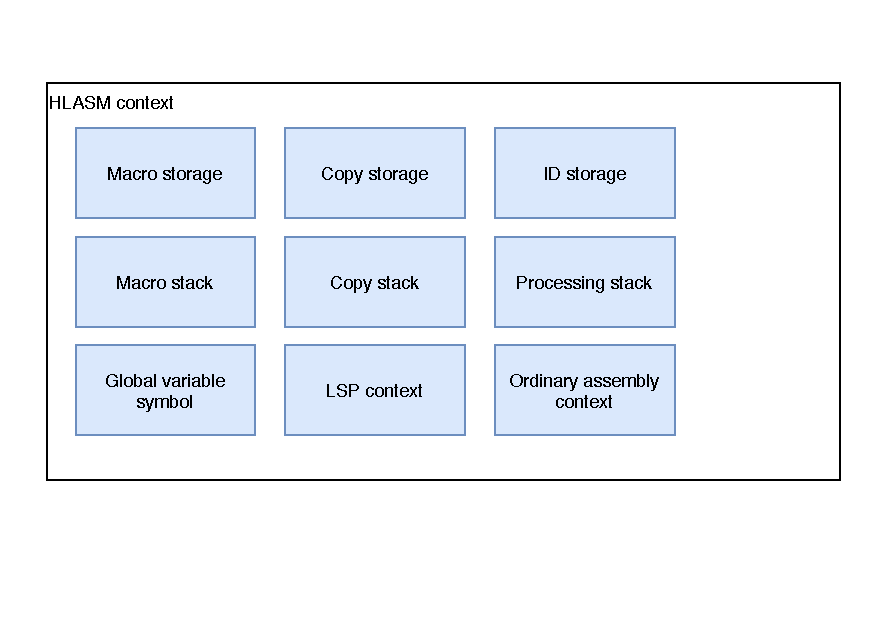
\includegraphics[width=\textwidth / 2]{img/hlasm_arch}
	\caption{The composition of HLASM context tables component}
	\label{fig06:hlasm}
\end{figure}

\subsection{Macros}

HLASM context stores visited macro definitions located in the \emph{macro strorage}. 

Macro definition is represented by:
\begin{enumerate}
	\item \emph{Macro name} --- to identify the macro.
	\item \emph{Calling parameters}. They are assigned real parameters when the macro is called.
	\item \emph{Block of statement}. Represents the body of the macro.
	\item \emph{Block of copy nestings}. It is array with one-to-one relation with block of statements. Each entry is a list of in-file locations that represents how much was the statement nested in COPY calls.
	\item \emph{Label storage}. The storage of sequence symbol that occur in the macro definition.
\end{enumerate}

When macro is called, \emph{macro invocation} object is created. It shares the content of a respective macro definition with an exception of calling parameters as they are assigned real value passed with the call. Also, it contains information which is the current statement in the invocation.

The macro invocation is stored in the context's \emph{scope stack}.

\subsection{Scope stack}

This stack holds information about the scope of variable symbols (see ??). The scope changes when macro is visited and the initial scope is the open-code. 
The stack contains:
\begin{itemize}
	\item In-scope variable symbols.
	\item In-scope sequence symbols.
	\item Pointer to the macro invocation (NULL if in open-code).
	\item Branch counter (for ACTR instruction).
\end{itemize}

\subsection{COPY}

HLASM context stores visited COPY members in the \emph{copy strorage}.

COPY member definition is much simpler as it does not hold any more semantic information than a peace of string.

When copy is visited, copy member invocation is created and pushed in the copy stack of last entry of the \emph{source stack}.

\subsection{Source stack and Processing stack}

This stacks are responsible for the nests of opened files (source stack) and what they are opened for (processing stack). As the relation of source entry and processing entry is one-to-many, the information is stored in two arrays rather than one.

When an statement processor (see \cref{lab06:sect_proc}) change (e.g. macro or copy definition is processed, lookahead is needed, ...), this information is stored in the processing stack. When, during the change, new file is opened then source stack is updated correspondingly.

Source stack contains copy stack active for a respective source file and data that locates last processed statement in the source file.
Processing stack contains \emph{processing kind}.

The reasoning of organizing this two stacks in such a way is:
\begin{enumerate}
	\item Context has enough information to fully reconstruct the statement.
	\item Easy retrieval of the correct copy stack for copy statement provider.
\end{enumerate} 

\subsection{ID storage}

ID storage holds the string identifiers that are used by the open-code. 
It stores the string and retrieves a pointer. It is guaranteed that if two different strings with the same value are passed to the storage, the resulting pointers are equal.

It simplifies work with IDs and saves space. 

\subsection{LSP context}

\subsection{Ordinary assembly context}

The above described structures aimed the high-level part of the language (code generation). As we move closer to the resulting object code of the source file, the describing structures get complicated. Therefore, HLASM context contains object storing just this part of the processing.

\begin{figure}
	\centering
	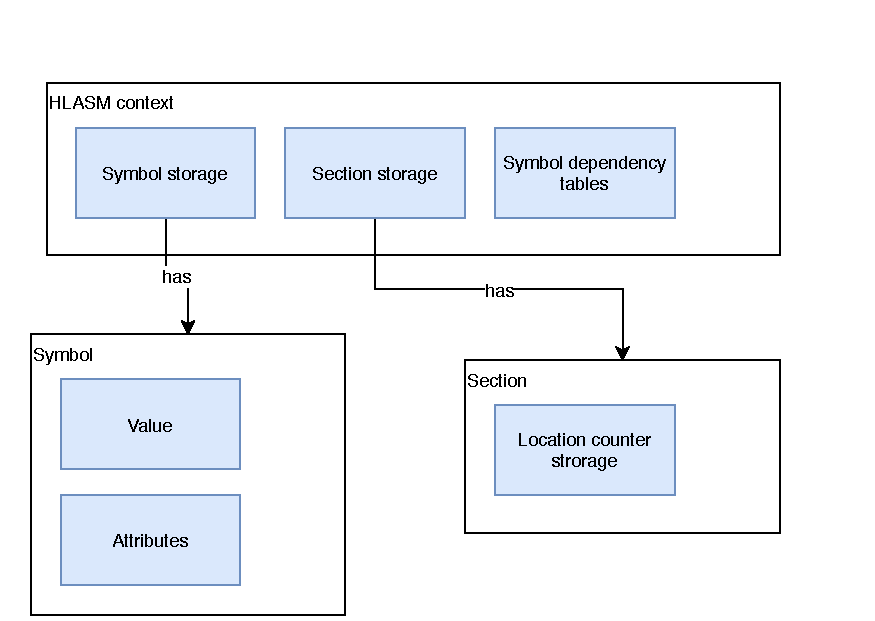
\includegraphics[width=\textwidth / 2]{img/ord_ctx_arch}
	\caption{The composition of Ordinary assembly context}
	\label{fig06:ord_ctx}
\end{figure}

Ordinary assembly context consists of three main components (see \cref{fig06:ord_ctx}):
\begin{enumerate}
	\item \emph{Symbol storage}. Stores ordinary symbols (see ??).
	\item \emph{Section storage}. Has notion of all generated sections, each section containing its location counters.
	\item \emph{Symbol dependency tables}. Contains yet unresolved dependencies between symbols prior to the currently processed instruction.
\end{enumerate}

\subsubsection{Symbol}

This class represents HLASM Ordinary symbol. Besides its identifier and location, symbol contains \emph{value} and \emph{attributes} components.

\paragraph*{Value} can be assigned \emph{absolute} or \emph{relocatable} values --- as the HLASM docs states. With addition to that, it can also be assigned empty value stating that symbol is not yet defined.

\paragraph*{Attributes} structure holds symbol attributes like type, length, scale and integer.

\subsubsection{Location counter}

As the location counter value handling is fairly complex in HLASM language, this class needed to be added to represent the location counter data of each section.


\paragraph*{Location counter data} is structure defining current value of the location counter. It consist of:
\begin{itemize}
	\item \emph{Storage} stating total number of bytes occupied by the location counter.
	\item Vector of \emph{spaces}, block of bytes with yet not known length.
	\item Vector of \emph{storage} between each space.
\end{itemize}

The location counter value with respect to the respective section is transformable into relocatable value. Structure that represents it is called \emph{address}.

\paragraph*{Address} consists of:
\begin{itemize}
	\item Array of \emph{bases}, sections that are points of reference for the address.
	\item Array of \emph{spaces} that are present in the address. 
	\item Total value of \emph{storage} as the offset from the bases.
\end{itemize}

The common composition of an address is one base section as the start of the address and value of storage as the offset from it.

The need for array of bases is there because addresses from different sections can be added or substracted. This information is needed as the correct sequence of arithmetic operations can reduce number of bases (even spaces) to zero and create absolute value. This value can be later used in places where a relocatable value would be forbidden.

\paragraph*{Space} is created when statement generating data with yet unknown length is encountered. It is stored in the current location counter. 

It contains an array of address listeners. Hence, when an address is assigned a relocatable value that contains space, the address is added to its array. This serves as a point of space resolving. Therefore, when the length that space represents becomes known, space is resolved and all its listeners are updated.

\vspace{0.5cm}

Location counter value can be arbitrarily changed and reverted back to its previous state with ORG instruction. Therefore, location counter holds an array of the location counter data to satisfy this requirement.

\subsubsection{Symbol dependency tables}

HLASM forbids cyclic symbol definition. However, user can still write it. Therefore, there is a need for maintaining dependencies between symbols.

Let us describe the main components of dependency resolving:

\paragraph*{Dependant} is a structure used in the symbol dependency tables that encapsulates objects that can be dependent on another objects. Currently it can be a symbol, symbol attribute or a space.

\paragraph*{Dependency solver} is an interface that can return value of the symbol providing its identifier. It is implemented by Ordinary assembly context.

\paragraph*{Dependable} If an object can contain dependencies, it implements \emph{dependable} interface. The interface has a method to retrieve an structure holding the respective dependants. 

\paragraph*{Resolvable} interface adds up to the dependable interface providing methods to return \emph{symbol value} with help of the dependency solver.

\vspace{0.5cm}

Map of dependencies has Dependable objects as keys and Resolvable objects as values. When new dependency \emph{D} is added, the map is checked in the following way:
\begin{enumerate}
	\item The resolvable object belonging to the dependency retrieves its dependencies.
	\item Dependencies are checked whether any of them is equal to \emph{D}. If yes, there is a dependency cycle. If no, start over for each dependency. 
\end{enumerate}

The reason for storing the resolvable object instead of an array of dependencies is that when some dependency gets resolved, the arrays would need to be updated. The resolvable object does not have this requirement.

Symbol dependency tables structure has maps serving as a dependency sources. They are sources of resolvable objects in dependency map. When a symbol dependency is created and added to the map, owning statement is stored there. This serves two purposes. Firstly, the statement cannot be checked as there are unresolved dependencies. Therefore, statement is postponed until its dependencies are resolved then passed to respective checker. Secondly, it prevents the observer Resolvable pointers to be inconsistent as the owning statement would be freed.